\documentclass[oneside]{ausarbeitung}
\bibliography{latexlit}


% ----------------------------------------------------------------------

\begin{document}

%--- Sprachauswahl
% Erlaubte Werte:
%   \selectlanguage{english}
%   \selectlanguage{ngerman}
\selectlanguage{ngerman}

%--- Art der Arbeit
% Erlaubte Werte:
%   \Praxissemesterbericht
%   \Projektbericht
%   \Bachelorarbeit
%   \Seminararbeit
%   \Masterarbeit

\Projektbericht

%--- Studiengang:
% Erlaubte Werte:
%   \Informatik
%   \Elektronik
%   \DataScience
\Informatik

\title{Erweiterung der Scavenger-Hunt-Webanwendung\\
um QR-Code-Funktionalität und UI/UX-Optimierungen}

\author{Fabian Dominik Wottke}
\matrikelnr{3003798}

%--- Ist der Erstbetreuer (\examinerA) an der Hochschule ein Professor?
% Erlaubte Werte:
%   \examinerIsAProfessortrue   % Ja
%   \examinerIsAProfessorfalse  % Nein
\examinerIsAProfessortrue   % Ja

%--- Betreuer
\examinerA{Dr.~Marc~Hermann}
%\examinerB{Prof.~Dr.~Ulrich~Klauck}

%--- Einreichungsdatum
\date{15. August 2026}

%--- Angaben zur Firma
% Auskommentieren, wenn die Arbeit nicht bei einer ext. Firma gemacht wurde.
%\companyname{Beispielfirma}
%\industrialsector{Beispielbranche}
%\department{Beispielabteilung}
%\companystreet{Beispielstr. 1}
%\companycity{12345 Musterstadt}

%--- Angaben zum Betreuer bei dieser Firma
%\advisorname{Dr.~Marc~Hermann}
%\advisorphone{(01234) 567-890}
%\advisoremail{name@company.xxx}

%--- Titelseite Anzeigen
\maketitle
\cleardoublepage

%---
\pagenumbering{roman}
\setcounter{page}{1}

%--- Firmendaten Anzeigen
% Auskommentieren, wenn die Arbeit nicht bei einer ext. Firma gemacht wurde.
%\makeworkplace
%\cleardoublepage

%--- Eidesstattliche Erklärung anzeigen
\makeaffirmation
\cleardoublepage

%--- Sperrvermerk (Funktioniert nur bei externen Bachelor- oder Masterarbeiten.)
%\makeconfidentialclause
%\cleardoublepage

%---
\begin{abstract}

  Im Rahmen dieser Projektarbeit wurde die bestehende Scavenger-Hunt-Webanwendung funktional und gestalterisch erweitert.
  Die Anwendung ermöglicht es Nutzern, ditigale Schnitzeljagden zu erstellen, zu verwalten und zu spielen.
  Ein besonderer Schwerpunkt der Arbeit lag auf der Verbesserung des Beitrittsprozesses sowie der Einführung einer neuen 
  Möglichtleit zur Antwortauswahl. Darüber hinaus stellte die Optimierung der Benutzeroberfläche und der Benutzererfahrung 
  (UI/UX) auch ein zentrales Ziel der Arbeit.

  Als zentrale funktionale Erweiterung wurde ein Qr-Code-Scanner entwickelt und in den bestehenden Join-Prozess integriert.
  Dadurch können Nutzer einer Hunt neben der manuellen EIngabe eines Hunt-Codes auch direkt über einen Qr-Code beitreten.
  Der Scanner verwendet die Browser-Schnittstelle MediaDevices für den Kamerazugriff und die Bibliothek jsQR zur Erkennung 
  und Dekodierung von QR-Codes. Zusätzlich wurden Funktionen wie die Auswahl eines QR-Code-Bildes aus der Galerie, der Wechsel 
  zwischen verfügbaren Kameras sowie eine umfassende Behandlung von Kamera-, Scan- und Eingabefehlern umgesetzt.

  Neben der QR-Code-Fuinktionalität wurde die Benutzeroberfläche der Anwendung üverarbeitet und insbesondere für die Nutzung
  auf mobilen Geräten optimiert. Hierzu wurden zentrale Seiten neu gestalltet, wiederverwendbare UI-Komponenten eingeführt
  sowie ein einheitliches Farbkonzept mit Light- und Dark-Mod umgesetzt. Darüber hinaus wurde die bestehende 
  Intenationaliesirung erweitert und die Anwendung für eine zusätzliche polnische Benutzeroberfläche vorbereitet.

  Die umgesetzten Erweiterungen verbessern insbesondere die Benutzerfreundlichkeit beim Beitritt zu einer Schnitzeljagd sowie
  die sowie die Konsistenz und mobile Nutzbarkeit der anwendung. die Ergebnisse werden anschließend anhand funktionaler Tests
  und einer Nutzerevalution bewertet.

  \begin{itemize}
    \item des in der Arbeit angegangenen Problems
    \item der verwendeten Methode(n)
    \item des in der Arbeit erzielten Fortschritts.
  \end{itemize}

  Dabei sollte nicht auf die Struktur der Arbeit eingegangen werden, also 
  Kapitel~\ref{cha:grundlagen} etc. denn die Kurzfassung soll ja gerade 
  das Wichtigste der Arbeit vermitteln, ohne dass diese gelesen werden muss.
  Eine Kapitelbezogene Darstellung sollte sich in Kapitel~%
  \ref{cha:einleitung} unter Vorgehen befinden.

  Länge: Maximal 1 Seite.
\end{abstract}
%-----------------------------------------------------------------------
\cleardoublepage
\tableofcontents

%---
\listoffigures

%---
\listoftables

%---
\lstlistoflistings

%---
\listofabbreviations
\begin{acronym}[MediaDevices]  % Längstes Kürzel in der nachfolgenden
                       % Liste um die Breite der Spalte für die
                       % Abkürzungen zu bestimmen.


%% Eintrag: \acro{Referenzname}[Kürzel]{Langform}
%% Im Text wird die Abkürzung dann mit \ac{Referenzname} benutzt.
  \acro{rup}[RUP]{Rational Unified Process}
  \acro{qr}[QR]{Quick Response}
  \acro{ui}[UI]{User Interface}
  \acro{ux}[UX]{User Experience}
  \acro{api}[API]{Application Programming Interface}
%\acro{bsp}[Bsp.]{Beispiel}
\end{acronym}
%---


\cleardoublepage
\pagenumbering{arabic}
\setcounter{page}{1}

% ----------------------------------------------------------------------
\chapter{Einleitung}
\label{cha:einleitung}

Die Einleitung dient dazu, beim Leser Interesse für die Inhalte 
Praxissemesterberichts zu wecken, die behandelten Probleme aufzuzeigen 
und die zu ihrer Lösung entwickelten Konzepte zu beschreiben.

\section{Motivation}
\label{sec:motivation}

Digitale Schnitzeljagden bieten die Möglichkeit, reale Orte mit interaktiven und multimedialen Aufgaben zu verbinden.
Die bestehende Scavenger-Hunt-Webanwendung der Vorherigen Projektarbeit (Sommer Semester 2025) der Hochschule Aalen ermöglicht es,
solche Schnitzeljagden zu erstellen und zu spielen. Dabei können unterscheidliche Aufgabentypen, Antwortmöglichkeiten und Hinweisarten
genutzt werden, welche durch Text-, Bild-, Video-, Audio- und GPS-Inhalte unterschieden werden können.
Dadurch eignet sich die Anwendung beispielsweise dazu, Orte und Angebote der Hochschule Aalen auf spielerische Weise zu erkunden oder
auch für andere Bildungseinrichtungen, wie Musseen oder Schulen.

Mit zunehmender Funktionsumfang steigen jedoch auch die Anforderungen an eine intuitive und mobil nutzbare Benutzeroberfläche, welche 
zudem auch einen eigenen wiedererkennbaren Stil aufweisen sollte. Insbesondere beim Einstieg in eine >Schnitzeljagd sollte der notwendige
INteraktionsaufwand möglichst gering gehalten werden. Die bisherige Eingabe eines Hunt-Codes stellt zwar eine funktionale Möglichkeit 
zum Beitritt dar, jedoch erfordet die manuelle Eingabe eines Codes und kann auf mobilen Endgeräten umständlich sein.

Die Integration eines QR-Scanners bitet hierfür eine direkte und für moblie Geräte geeignete Möglichkeit zum Beitritt zu einer Schnitzeljagd.
Ein bereitgestellter QR-Code kann mit der Gerätekamera gescannt werden und die darin enthaltene Information unmittelbar für den Beitrittsporzess
verwendet werden. Jedoch wird die IMplementierung eines solchen Scanners auch für die Antwortmöglichkeit bei den Aufgaben verwendet, sodass man
gezielt einen von der Anwendung generierten QR-Code ausdrucken und verstecken kann und im späteren Verlauf auch gefunden und gescannt werden kann.
Neben diesen Funktionalen Erweiterungen besteht die Motivation der Arbeit darin, die bestehende Benutzerpberfläche hinsichtlich Konsistenz, 
Verständlichkeit und responsiver Darstellung weiterzuentwickeln.

Ziel der Erweiterung ist es damit, bestehende Funktionen der Scavenger-Hunt-Anwendung leichter zugänglich zu machen und gleichzeitig eine 
einheitliche Benutzererfahrung auf Desktop und Mobilgeräten zu schaffen.

\section{Problemstellung und -abgrenzung}
\label{sec:problemstellung}

Die Scavenger-Hunt-Anwendung stellte zu Beginn dieser Projektarbeit bereits wesentliche Funktionen zum Erstellen, Verwatlen und Spielen digitaler
Schnitzeljagden bereit. Im Rahmen der Einarbeitung zeigten sich jedoch sowohl funktionale als auch strukturelle und gestalterische 
Verbesserungspotenziale.

Ein zentrales Verbesserungspotenzial der bestehenden Scavenger-Hunt-Anwendung bestand bei der Nutzung von QR-Codes. Der Beitritt zu einer Hunt
sollte über einen direkt in die Webanwendung integrierten QR-Code-Scanner vereinfacht werden, dieselbe Funktionalität des QR-Code-Scanners sollte 
auch bei entsprechenden Aufgaben innerhalb einer Hunt wiederverwendet werden. Dadurch können QR-Codes beispielsweise als Antwortmöglichkeit 
für einzelne Stationen eingesetzt werden.

Neben dieser funktionalen Erweiterung zeigten sich bei der Einarbeitung in das bestehende Projekt auch Verbesserungspotenziale hinsichtlich 
der Benutzeroberfläche. Die Gestaltung der Anwendung wirkte auf vielen Seiten sehr zurückhaltend und war durch einen hohen Anteil weißer Flächen 
geprägt. Dadurch entstand teilweise ein visuell wenig differenziertes Erscheinungsbild, welches auch keinen wiedererkennbaren Stil aufwies, welcher
die Anwendung leichter erkennbar machen würde. Dieser Eindruck wurde auch im Rahmen einer Besprechung mit dem Betreuer thematisiert, wobei 
insbesondere der starke Weißanteil der bestehenden Oberfläche als Verbesserungspotenzial identifiziert wurde.

Darüber hinaus war beispielsweise die Bearbeitung einer Hunt teilweise unübersichtlich, da Funktionen und Informationen auf der Seite zunächst 
gesucht werden mussten. Ziel war daher nicht nur eine farbliche Überarbeitung, sondern auch eine klarere visuelle Hierarchie und eine konsistentere 
Gestaltung der verschiedenen Seiten um ein leichteres Verständnis un eine bessere Orientierung für den Benutzer zu garantieren.

Auch die Struktur des Frontend-Codes erschwerte teilweise die Einarbeitung und zukünftige Weiterentwicklung. Obwohl der bestehende Quellcode 
kommentiert war, befanden sich zahlreiche Seitenelemente und zugehörige Gestaltungsregeln direkt innerhalb einzelner Seiten beziehungsweise deren 
CSS-Dateien. Wiederkehrende Elemente, beispielsweise Buttons und deren Farbdefinitionen, waren dadurch teilweise mehrfach oder seitenbezogen 
umgesetzt, obwohl sie an verschiedenen Stellen der Anwendung verwendet wurden. Dies führte zu größeren Dateien und machte es notwendig, für Änderungen 
zunächst nach den jeweiligen Definitionen zu suchen.

Im Rahmen dieser Arbeit wurde daher ein Teil dieser wiederkehrenden Strukturen zentralisiert. Wiederverwendbare Bedienelemente wurden teilweise
in eigene Komponenten ausgelagert, welche sich in den dazugehörigen passenden Ordnern befinden, und zentrale Gestaltungswerte, insbesondere Farben, 
an einer gemeinsamen Stelle (App.css) definiert und kommentiert. Dadurch sollen Anpassungen leichter nachvollziehbar sein und die visuelle Konsistenz 
zwischen den Seiten verbessert werden.

Der Schwerpunkt der Arbeit liegt somit auf der funktionalen Erweiterung um eine wiederverwendbare QR-Code-Scan-Funktionalität, der Verbesserung 
der Benutzerführung sowie einer gezielten Überarbeitung und Vereinheitlichung der Benutzeroberfläche. Eine vollständige Restrukturierung der gesamten 
bestehenden Codebasis sowie eine grundlegende Neuentwicklung der Hunt-, Benutzer- oder Spiellogik sind dagegen nicht Bestandteil dieser Arbeit und 
würden den Rahmen der Arbeit sprengen.

\section{Ziel der Arbeit}
\label{sec:ziel}

Das Ziel der Arbeit besteht darin, die bestehende Scavenger-Hunt-Webanwendung funktional und gestalterisch weiterzuentwickeln. Der Schwerpunkt liegt 
dabei auf der Entwicklung und INtegration eines wiederverwendbaren QR-Code-Scanners, der sowohl für den Beitritt zu einer Hunt als auch für die 
Beantwortung von Aufgaben innerhalb einer Hunt verwendet werden kann.

Der Scanner soll direkt im Browser funktionieren und den Zugriff auf die Kamera eines Geräts ermöglichen. Neben der Erkennung von QR-Codes über 
einen laufenden Kamerastream soll auch das Auslesen eines bereits vorhandenen QR-Code-Bildes aus der Galerie unterstützt werden. Darüber hinaus 
sollen auch unterschiedliche Kameras eines Geräts ausgewählt sowie typische Fehlerfälle, beispielsweise fehlende Kamera oder fehlende Berechtigungen,
verständlich behandelt werden.

Ein weiteres Ziel der Arbeit ist die Verbesserung der Benutzeroberfläche und der Benutzererfahrung. Die Anwendung soll insbesondere auf mobilen 
Endgeräten übersichtlicher und einfacher bedienbar werden. Hierzu werden ausgewählte Seiten hinsichtlich Struktur, responsiver Darstellung, visueller 
Hierarchie und einheitlicher Gestaltung überarbeitet um eine bessere Orientierung und ein konsistenteres Erscheinungsbild zu schaffen. Zusätzlich soll
das bestehende Farbkonzept vereinheitlicht und um einen konsistenten Light- und Dark-Mode ergänzt werden, welches wiederrum auch die visuelle Konsistenz 
der Anwendung verbessern soll.

Zur Verbesserung der Wartbarkeit sollen außerdem ausgewählte wiederkehrende Bestandteile des Frontends zentralisiert und wiederverwendbar gestaltet werden. 
Dazu gehören insbesondere gemeinsam verwendete Bedienelemente sowie zentrale Farb- und Gestaltungsdefinitionen, jedoch soll auch verhindert werden, dass
eine komplette Restrukturierung des bestehenden Frontend-Codes notwendig ist.

Abschließend sollen die umgesetzten Erweiterungen sowohl durch funktionale Tests als auch durch eine Nutzerevaluation überprüft werden. Dabei wird 
untersucht, ob die neuen Funktionen verständlich bedienbar sind und ob die überarbeitete Gestaltung gegenüber dem zuvor bestehenden Zustand eine 
Verbesserung der Benutzererfahrung darstellt.



\section{Vorgehen}
\label{sec:vorgehen}

Nachdem mit Problemstellung und Ziel gewissermaßen Anfangs- und Endpunkt 
des Praktikums beschrieben sind, wird hier der zur Erreichung des Ziels 
eingeschlagene Weg vorgestellt. Dazu werden typischerweise die folgenden 
Kapitel und ihr Beitrag zur Erreichung des Ziels der Arbeit kurz 
beschrieben. Die folgenden Kapitel sind ein – möglicher – Aufbau, 
Abweichungen können durchaus notwendig sein. Zur Darstellung des 
Vorgehens ist eine grafische Darstellung sinnvoll, bei der die einzelnen 
Lösungsschritte und ihr Zusammenhang dargestellt werden. 


Zu Beginn der Projektarbeit wurde vom Betreuer die Erweiterung der bestehenden Scavenger-Hunt-Anwendung um eine QR-Code-Funktionalität als zentrale
Aufgabe vorgeschlagen. Daraufhin erfolgte zunächst eine Einarbeitung in die bestehende Anwendung und insbesondere in den vorhandenen Beitrittsprozess 
zu einer Hunt. Dabei wurde untersucht, wie der bestehende Beitrittsprozess funktioniert, welche Daten übermittelt werden und wie ein QR-Code-Scanner
in den bestehenden Prozess integriert werden kann. Parallel dazu wurde eine Recherche zu bestehenden QR-Code-Scanner-Bibliotheken durchgeführt und
wie man diese Bibiotheken sinnvoll verwendet und in die bestehende Anwendung integriert.

Auf Grundlage dieser Einarbeitung und Recherche wurden erste Lösungsansätze für die QR-Code-Integration sowie weitere mögliche Verbesserungen der 
Anwendung entwickelt. Die grundlegenden Ziele und der geplante Umfang der Projektarbeit wurden anschließend mit dem Betreuer abgestimmt. 
Aus diesen Vorgaben wurden die Anforderungen im nächsten Schritt eigenständig priorisiert und in Must-Have-, Should-Have-, Could-Have- und 
Nice-To-Have-Anforderungen eingeordnet. Diese Priorisierung diente im weiteren Projektverlauf als grobe Orientierung für die Umsetzung und Abgrenzung 
der einzelnen Erweiterungen.

Anschließend wurde weiter recherchiert, wie ein QR-Code-Scanner innerhalb einer Webanwendung technisch umgesetzt werden kann. Dabei wurden verschiedene 
mögliche Ansätze und Bibliotheken betrachtet. Zu Beginn wurde unter anderem die Bibliothek html5-qrcode als mögliche Lösung in Betracht gezogen, jedoch 
war auch die Bibliothek @zxing/browser eine mögliche Alternative, die jedoch aufgrund der Komplexität und des höheren Aufwands für die Integration 
in die bestehende Anwendung zunächst nicht weiter verfolgt wurde. Zu dem wurden auch Ansätze für die Überarbeitung der Benutzeroberfläche bedacht,
insbesondere die Einführung eines konsistenten Farbkonzepts und die Verbesserung des Designs der wichtigsten Seiten und im weiteren mit dem Betreuer 
festgelegt. 

Im folgenden Schritt wurde ein Prototyp für die QR-Code-Integration mit Hilfe der html5-qrcode-Bibliothek entwickelt. Dabei wurde zunächst ein einfacher
QR-Code-Scanner implementiert, der die Kamera eines Geräts verwendet und QR-Codes erkennen kann. Jedoch zeigte sich, dass diese Implementierung nicht
der erwarteten Niveau und Umfang der Projektarbeit entsprach, sodass im weiteren Verlauf eine weitere Recherche zu alternativen Bibliotheken durchgeführt
wurde, wodurch die Bibliothek jsQR als geeignete Lösung identifiziert wurde. Diese Bibliothek ermöglicht eine direkte Verarbeitung von Kamerastreams und
eine bessere, kontrolierbare und flexiblere Integration in die bestehende Anwendung. Daraufhin wurde der alte Prototyp erstmallig als Notlösung betrachtet,
falls der Prototyp mit der jsQR-Bibliothek nicht Erwartungsgemäß funktioniert. 

Daraufhin wurde ein neuer Prototyp mit der jsQR-Bibliothek entwickelt, der die Kamera eines Geräts verwendet und QR-Codes erkennen kann und auch schon die 
groben Design-Erwartungen an die spätere Integration in die bestehende Anwendung entsprach. Daraufhin wurde eine weitere Abstimmung mit dem Betreuer 
durchgeführt, bei der die geplante Überarbeitung der Benutzeroberfläche leicht konkretisiert wurden und weitere mögliche Verbesserungen des QR-Codes-Scanners
besprochen wurden, wie beispielsweise die Möglichkeit, ein QR-Code-Bild aus der Galerie auszuwählen und zu scannen, mehrere Kameras eines Geräts auszuwählen
und die genauere Spezifikation typischer Fehlerfälle, wie fehlende Kamera oder fehlende Berechtigungen, verständlich zu behandeln. Aber auch wurde eine weitere 
erstmals im Hintergrund vergessene Anforderung besprochen, dass der QR-Code-Scanner auch für die Beantwortung von Aufgaben innerhalb einer Hunt wiederverwendet 
werden sollten.

Im weiteren Verlauf der Projektarbeit wurde der Prototyp des QR-Code-Scanners weiterentwickelt und um die besprochenen Funktionen erweitert. Dabei wurde auch
die Integration der Erweiterung der bestehenden Fehlerfälle und deren Behandlung, aber auch die Integration in die Hunt-Beantwortung prioritisiert und 
umgesetzt. Anschließend wurden auch die anderen Funktionen, wie die Auswahl eines QR-Code-Bildes aus der Galerie und die Auswahl einer Kamera implementiert. 
Anschließend wurde auch die Benutzeroberfläche der Anwendung überarbeitet, insbesondere die wichtigsten Seiten, wie die Startseite, die Hunt-Übersichtsseite
und die Hunt-Bearbeitungsseite. Dabei wurden wiederverwendbare UI-Komponenten eingeführt, zentrale Farbdefinitionen in einer gemeinsamen Datei (App.css) definiert 
und die bestehende Internationalisierung erweitert, sodass die Anwendung auch für eine polnische Benutzeroberfläche vorbereitet ist.

Nach Abschluss der wesentlichen Implementierungsarbeiten wurden die neuen Funktionen sowie die überarbeitete Benutzeroberfläche funktional getestet. Zusätzlich 
wurde eine Nutzerevaluation durchgeführt, um insbesondere die Verständlichkeit der Bedienung und die Wahrnehmung der überarbeiteten Oberfläche zu untersuchen.

Abschließend werden die umgesetzten Ergebnisse mit den zu Beginn definierten Anforderungen verglichen und hinsichtlich ihrer Zielerreichung bewertet. Nicht oder 
nur teilweise realisierte Anforderungen werden dabei ebenfalls dokumentiert und als mögliche Ansatzpunkte für zukünftige Erweiterungen betrachtet.

%\begin{figure}[htbp]
%  \centering
%  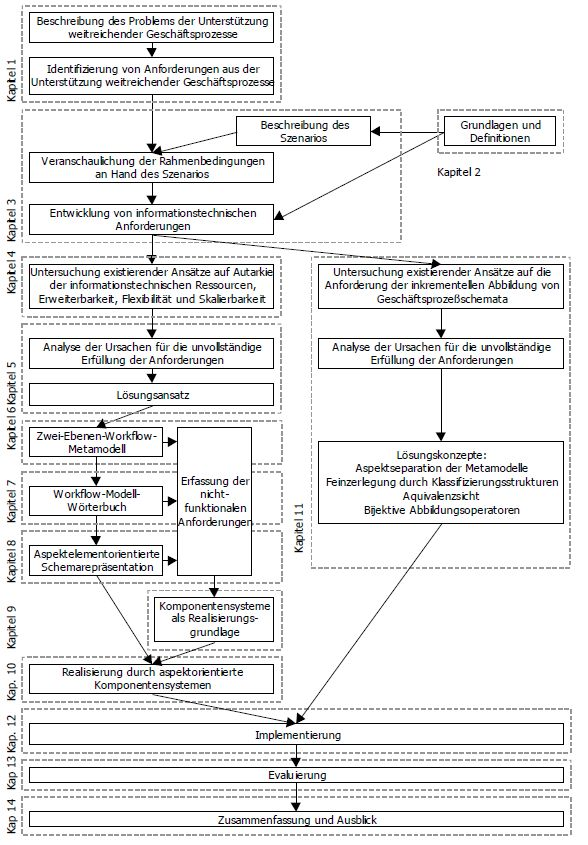
\includegraphics[height=0.9\textheight]{images/ausarbeitung.jpg}
%  \caption{vorgehen nach \autocite{Schmidt:Geschaeftsprozesse}}
%  \label{fig:1}
%\end{figure}


% ---
\chapter{Grundlagen}
\label{cha:grundlagen}

In diesem Kapitel das für das Praktikum relevante Grundlagenwissen 
dargestellt. Der Praktikant soll hierzu das ihm durch Vorlesungen 
bekannte, bzw. durch Recherchen vertiefte theoretische Wissen 
darstellen, das für die Lösung der im Praktikum gestellten Probleme 
notwendig ist.

Dabei ist darauf zu achten, nur solche Inhalte in das Grundlagenkapitel 
aufzunehmen, die später auch verwendet werden (Problembezogenheit). 
Ebenso ist auf eine ausreichend tiefe und vollständige Darstellung der 
Grundlagen zu achten.

Für die Erstellung des Literaturverzeichnisses 
wird das Werkzeug JabRef\autocite{JabRef:JabRef} verwendet. 

Sie können aber auch das Werkzeug Citavi\autocite{SAS:Citavi} benutzen
und dort nach \textsc{Bib}\TeX{} exportieren.

\section{Grundlagengebiet A}
\label{sec:grundlagengebieta}

\blindtext

\subsection{Definition AA}
\label{sub:definitionaa}

\blindtext

\subsection{Definition AB}
\label{sub:definitionab}

\blindtext

\section{Grundlagengebiet B}
\label{sec:grundlagengebietb}

\blindtext

\subsection{Definition BA}
\label{sub:definitionBa}

\blindtext

\subsection{Definition BB}
\label{sub:definitionbb}

\blindtext

%---
\chapter{Problemanalyse}
\label{cha:problemanalyse}

Die Analyse des zu lösenden Problems ist Grundlage für jedes 
ingenieurmäßige Vorgehen. Daher soll in diesem Kapitel das zu lösenden 
Problem auf Basis des im Grundlagenkapitel aufbereiteten Wissens 
analysiert werden. Hierzu ist insbesondere notwendig zu klären, wie sich 
das Gesamtproblem in Teilprobleme zerlegen lässt und welche 
Abhängigkeiten zwischen diesen bestehen.

Bei Software-Projekten befindet sich an dieser Stelle typischerweise die 
Anforderungsanalyse des \ac{rup}.

%---
\chapter{Lösungskonzept}
\label{cha:loesungskonzept}

Auf der Basis der im vorangegangenen Kapitel erstellten Problemanalyse 
und der im Grundlagenkapitel aufgearbeiteten theoretischen Kenntnisse 
wird ein Lösungskonzept erarbeitet.

Bei Software-Projekten entspricht dieses Kapitel typischerweise der 
Analyse \& Design-Phase des \ac{rup}. Typische Ergebnisse dieser Phase sind 
Klassendiagramme etc.

%---
\chapter{Implementierung}
\label{cha:implementierung}

In diesem Kapitel wird die konkrete Implementierung des im Kapitel
\ref{cha:loesungskonzept} entwickelten Lösungskonzepts beschrieben.
Hierbei wird auf die konkret verwendeten Entwicklungswerkzeuge etc. 
Bezug genommen.

Bei Software-Projekten besteht dieses Kapitel typischerweise aus den 
Phasen Implementierung \& Test im \ac{rup}.

Zum Beispiel kann man hier auch ein kleines Listing einfügen (Siehe \ref{lst:test}).

\begin{lstlisting}[language=c,%
                   caption={Überschrift des Quelltexts},label=lst:test]
#include<stdio.h>

int main() {
    // Kommentar
    int answer = 20 << 1;
    answer += 2;
    printf("Hallöchen Welt!\n");
    printf("Die Antwort ist: %d\n", answer);
    return 0;
}
\end{lstlisting}

Manchmal hilft auch eine kleine Tabelle:

\begin{table}[htbp]
\centering
\begin{tabular}{|l|r|}
\hline
\textbf{Messwert a} & \textbf{Messwert b} \\ \hline
9 & 5 \\ \hline
1 & 4 \\ \hline
1 & 3 \\ \hline
\end{tabular}
\caption{Überschrift der Tabelle}
\label{tab:my-table}
\end{table}

Details siehe Tabelle~\ref{tab:my-table}.
%---
\chapter{Inbetriebnahme}
\label{cha:inbetriebnahme}

Aufgabe des Kapitels Inbetriebnahme ist es, die Überführung der in 
Kapitel \ref{cha:implementierung} entwickelte Lösung in das betriebliche 
Umfeld aufzuzeigen. Dabei wird beispielsweise die Inbetriebnahme eines 
Programms beschrieben oder die Integration eines erstellten 
Programmodules dargestellt.

Bei der Software-Erstellung entspricht dieses Kapitel der 
Auslieferungsphase (Deployment) im \ac{rup}.

%---
\chapter{Evaluierung}

Aufgabe des Kapitels Evaluierung ist es, in wie weit die Ziele der 
Arbeit erreicht wurden. Es sollen also die erreichten Arbeitsergebnisse 
mit den Zielen verglichen werden. Ergebnis der Evaluierung kann auch 
sein, das bestimmte Ziele nicht erreicht werden konnten, wobei die 
Ursachen hierfür auch außerhalb des Verantwortungsbereichs des 
Praktikanten liegen können.

%---
\chapter{Zusammenfassung und Ausblick}
\label{cha:zusammenfassung}

\section{Erreichte Ergebnisse}
\label{sec:ergebnisse}

Die Zusammenfassung dient dazu, die wesentlichen Ergebnisse des 
Praktikums und vor allem die entwickelte Problemlösung und den 
erreichten Fortschritt darzustellen. (Sie haben Ihr Ziel erreicht und 
dies nachgewiesen).

\section{Ausblick}
\label{sec:ausblick}

Im Ausblick werden Ideen für die Weiterentwicklung der erstellten Lösung 
aufgezeigt. Der Ausblick sollte daher zeigen, dass die Ergebnisse der 
Arbeit nicht nur für die in der Arbeit identifizierten Problemstellungen 
verwendbar sind, sondern darüber hinaus erweitert sowie auf andere 
Probleme übertragen werden können.

\subsection{Erweiterbarkeit der Ergebnisse}
\label{sub:erweiterbarkeit}

Hier kann man was über die Erweiterbarkeit der Ergebnisse sagen.

\subsection{Übertragbarkeit der Ergebnisse}
\label{sub:uebertragbarkeit}

Und hier etwas über deren Übertragbarkeit.

%-----------------------------------------------------------------------
\appendix

%---
\printbibliography[heading=bibintoc]

%---
\chapter{Anhang A}

\Blindtext

%---
\chapter{Anhang B}

\Blindtext

\end{document}